% ==========================================
% CHAPITRE 4
% ==========================================
\newpage
\chapter{Étude et Réalisation du Deuxième Sprint}
\vspace{2.5cm}

\noindent \textbf{\Large Plan}
\vspace{0.8cm}

\begin{enumerate}[label=\textbf{\arabic*}, leftmargin=1.5cm, labelsep=0.8cm]
    \item[] \hspace*{-1.5cm}\textbf{Introduction}                          \dotfill \pageref{sec:s2-intro}
    \item \textbf{User Stories du deuxième sprint}       \dotfill \pageref{sec:s2-userstories}
    \item \textbf{Backlog du deuxième Sprint}            \dotfill \pageref{sec:s2-backlog}
    \item \textbf{Spécification fonctionnelle}           \dotfill \pageref{sec:s2-specification}
    \item \textbf{Conception du deuxième Sprint}         \dotfill \pageref{sec:s2-conception}
    \item \textbf{Étude et réalisation}                  \dotfill \pageref{sec:s2-realisation}
    \item \textbf{Tests et Validation}                   \dotfill \pageref{sec:s2-tests}
    \item \textbf{Rituels Agiles et Clôture du Sprint}   \dotfill \pageref{sec:s2-rituels}
    \item[] \hspace*{-1.5cm}\textbf{Conclusion}                            \dotfill \pageref{sec:s2-conclusion}
\end{enumerate}

\vfill
\newpage

% ============================================================
\section*{Introduction}
\label{sec:s2-intro}
\addcontentsline{toc}{section}{Introduction}
% ============================================================

S'appuyant sur les bases techniques consolidées lors du premier sprint, ce chapitre expose les réalisations du Sprint 2, véritable pivot opérationnel de la plateforme PaieZone RH. Cette itération est dédiée à la gestion du capital humain, intégrant l'administration des dossiers collaborateurs, le pilotage des cycles contractuels et la dématérialisation des documents administratifs. La méthodologie demeure rigoureuse : elle s'articule autour de la spécification par User Stories, d'une modélisation UML approfondie (classes et séquences), du développement des interfaces Angular, et se conclut par une phase de validation stricte suivie des rituels agiles de clôture.

% ============================================================
\section{User Stories du deuxième sprint}
\label{sec:s2-userstories}
% ============================================================

Lors de la réunion de planification du Sprint~2, l'équipe Scrum a défini
l'objectif du sprint autour de la valeur métier suivante~: «~Permettre à
l'équipe RH de gérer l'intégralité du dossier administratif d'un employé,
de son recrutement à la formalisation de sa relation contractuelle~». Trois
épics prioritaires ont été sélectionnés dans le backlog produit~:

\begin{itemize}[label=\textbullet, leftmargin=0.6cm]
    \item Gestion du Capital Humain
    \item Gestion du Cycle de Vie des Contrats de Travail
    \item Gestion des Documents Administratifs
\end{itemize}

Les besoins fonctionnels ont été formalisés sous forme de User Stories
détaillées dans le Tableau~\ref{tab:user-stories-sprint2}.
\renewcommand{\arraystretch}{1.4}
\begin{small}
\begin{longtable}{|p{1.2cm}|p{9.5cm}|p{2.3cm}|}

\hline
\rowcolor[gray]{0.9}
\textbf{ID} & \textbf{User Story} & \textbf{Priorité} \\
\hline
\endfirsthead

\hline
\rowcolor[gray]{0.9}
\textbf{ID} & \textbf{User Story} & \textbf{Priorité} \\
\hline
\endhead

\hline
\endfoot
\endfoot

6.1 & En tant qu'Admin/RH, je veux consulter la liste des employés,
      afin d'avoir une vue d'ensemble du personnel.
    & Haute \\ \hline

6.2 & En tant qu'Admin/RH, je veux créer un employé, afin de l'ajouter
      au système avec toutes ses données administratives et fiscales.
    & Critique \\ \hline

6.3 & En tant qu'Admin/RH, je veux consulter le profil d'un employé,
      afin de voir son dossier complet (informations, contrats,
      documents, historique).
    & Haute \\ \hline

6.4 & En tant qu'Admin/RH, je veux modifier un employé, afin de mettre
      à jour ses données personnelles ou contractuelles.
    & Haute \\ \hline

6.5 & En tant qu'Admin/RH, je veux désactiver un employé, afin de
      gérer sa sortie de l'organisation.
    & Haute \\ \hline

7.1 & En tant que RH, je veux associer un contrat à un employé, afin
      de formaliser la relation de travail (CDI, CDD, CIVP, KARAMA,
      Intérimaire ou Stage).
    & Critique \\ \hline

7.2 & En tant que RH, je veux modifier un contrat, afin de mettre à
      jour ses conditions avant résiliation.
    & Haute \\ \hline

7.3 & En tant que RH, je veux résilier un contrat, afin de terminer
      formellement une relation de travail.
    & Haute \\ \hline

8.1 & En tant que RH, je veux déposer un document administratif dans
      le dossier d'un employé, afin de constituer son dossier numérique.
    & Moyenne \\ \hline
\caption{User Stories du deuxième Sprint}   
\label{tab:user-stories-sprint2}    
\end{longtable}
\end{small}
\renewcommand{\arraystretch}{1.0}

% ============================================================
\section{Backlog du deuxième Sprint}
\label{sec:s2-backlog}
% ============================================================

Le Backlog du produit est formalisé en User Stories organisées
par thèmes fonctionnels. Le Tableau~\ref{tab:backlog-sprint2} détaille ce
backlog pour le deuxième sprint, incluant les tâches techniques et leurs
estimations en jours.

\begin{small}
\renewcommand{\arraystretch}{1.4}
\setlength{\LTleft}{\fill}
\setlength{\LTright}{\fill}
\begin{longtable}{|p{2.5cm}|p{6.0cm}|p{6.0cm}|c|}
\hline
\rowcolor[gray]{0.9} \textbf{Item} & \textbf{User Story} & \textbf{Tâches} & 
\makecell{\textbf{Est.}\\\textbf{(j)}} \\ \hline
\endfirsthead

\hline
\rowcolor[gray]{0.9} \textbf{Item} & \textbf{User Story} & \textbf{Tâches} & 
\makecell{\textbf{Est.}\\\textbf{(j)}} \\ \hline
\endhead
\hline
\endfoot
\hline
\caption{Backlog détaillé du deuxième Sprint}
\label{tab:backlog-sprint2}
\endlastfoot
% ── Gestion du Capital Humain ─────────────────────────────
\multirow{5}{*}{\makecell[c]{\textbf{Gestion du}\\ \textbf{Capital}\\ \textbf{Humain}}}
& \textbf{6.1} En tant qu'Admin/RH, je souhaite consulter la liste des
  employés afin d'avoir une vue d'ensemble du personnel.
& \begin{itemize}[leftmargin=*, noitemsep, topsep=0pt]
    \item Concevoir l'interface de la liste des employés (tableau paginé
          avec filtres et recherche).
    \item Développer l'API REST de récupération des employés liés à la
          société.
  \end{itemize}
& \textbf{1} \\ \cline{2-4}

& \textbf{6.2} En tant qu'Admin/RH, je souhaite créer un employé afin
  de l'ajouter au système.
& \begin{itemize}[leftmargin=*, noitemsep, topsep=0pt]
    \item Développer le formulaire de création du profil employé
          (informations personnelles, données fiscales et sociales,
          poste, département).
    \item Implémenter la génération automatique du matricule unique.
    \item Développer l'API REST d'insertion de l'employé.
  \end{itemize}
& \textbf{2} \\ \cline{2-4}

& \textbf{6.3} En tant qu'Admin/RH, je souhaite consulter le profil
  d'un employé afin de voir ses informations détaillées.
& \begin{itemize}[leftmargin=*, noitemsep, topsep=0pt]
    \item Implémenter la vue détaillée du profil employé (informations,
          contrats, documents, historique).
    \item Développer l'API REST de récupération du profil complet.
  \end{itemize}
& \textbf{1} \\ \cline{2-4}

& \textbf{6.4} En tant qu'Admin/RH, je souhaite modifier un employé
  afin de mettre à jour ses données.
& \begin{itemize}[leftmargin=*, noitemsep, topsep=0pt]
    \item Créer l'interface de modification du profil employé.
    \item Implémenter la mise à jour des données en base.
  \end{itemize}
& \textbf{1} \\ \cline{2-4}

& \textbf{6.5} En tant qu'Admin/RH, je souhaite désactiver un employé
  afin de gérer sa sortie de l'organisation.
& \begin{itemize}[leftmargin=*, noitemsep, topsep=0pt]
    \item Implémenter la logique de désactivation du profil.
    \item Gérer la désactivation du compte utilisateur associé.
    \item Tester l'impact sur les contrats actifs et les accès.
  \end{itemize}
& \textbf{1} \\ \hline

% ── Gestion des Contrats de Travail ──────────────────────
\multirow{3}{*}{\makecell[c]{\textbf{Gestion des}\\ \textbf{Contrats}\\ \textbf{de Travail}}}
& \textbf{7.1} En tant que RH, je souhaite associer un contrat à un
  employé afin de formaliser la relation de travail.
& \begin{itemize}[leftmargin=*, noitemsep, topsep=0pt]
    \item Concevoir l'interface de création et d'association d'un contrat.
    \item Implémenter les six types de contrats tunisiens~:
          \textbf{CDI}, \textbf{CDD} (date de fin obligatoire),
          \textbf{CIVP} (durée max.~1~an), \textbf{KARAMA},
          \textbf{Intérimaire}, \textbf{Stage} avec leurs règles de
          gestion spécifiques.
    \item Développer l'API REST de création de contrat.
    \item Implémenter la contrainte d'unicité~: un seul contrat actif
          par employé à un instant donné.
  \end{itemize}
& \textbf{2} \\ \cline{2-4}

& \textbf{7.2} En tant que RH, je souhaite modifier un contrat afin
  de mettre à jour ses conditions.
& \begin{itemize}[leftmargin=*, noitemsep, topsep=0pt]
    \item Créer l'interface de modification du contrat (formulaire
          pré-rempli).
    \item Implémenter la mise à jour des données du contrat.
    \item Tester les transitions de statut et la cohérence des dates.
  \end{itemize}
& \textbf{1.5} \\ \cline{2-4}

& \textbf{7.3} En tant que RH, je souhaite résilier un contrat afin
  de terminer une relation de travail.
& \begin{itemize}[leftmargin=*, noitemsep, topsep=0pt]
    \item Développer la logique de résiliation (motif obligatoire,
          date effective).
    \item Implémenter le passage du statut \texttt{ACTIF} à
          \texttt{RÉSILIÉ} en base.
    \item Tester le blocage de toute modification post-résiliation.
  \end{itemize}
& \textbf{1.5} \\ \hline

% ── Gestion des Documents Administratifs ─────────────────
\multirow{1}{*}{\makecell[c]{\textbf{Gestion des}\\ \textbf{Documents}\\ \textbf{Administratifs}}}
& \textbf{8.1} En tant que RH, je souhaite déposer un document afin
  de le stocker dans le dossier de l'employé.
& \begin{itemize}[leftmargin=*, noitemsep, topsep=0pt]
    \item Concevoir l'interface de dépôt et de consultation des
          documents du dossier.
    \item Développer le service de stockage de fichiers (PDF, images)
          avec gestion des types de documents.
    \item Implémenter les contrôles d'accès selon le rôle.
    \item Tester le dépôt, la consultation et la validation des formats.
  \end{itemize}
& \textbf{3} \\ \hline

\end{longtable}
\end{small}
\renewcommand{\arraystretch}{1.0}
\normalsize

% ============================================================
\section{Spécification fonctionnelle du deuxième Sprint}
\label{sec:s2-specification}
% ============================================================

La modélisation fonctionnelle du Sprint~2 repose sur des diagrammes de
cas d'utilisation UML, offrant une représentation visuelle du périmètre
fonctionnel, complétés par des descriptions textuelles structurées
détaillant les scénarios d'interaction pour chaque cas d'utilisation
majeur.

% -----------------------------------------------------------
\subsection{Diagramme de cas d'utilisation du deuxième Sprint}
% -----------------------------------------------------------

La Figure~\ref{fig:use-case-sp2} présente le diagramme de cas
d'utilisation global du Sprint~2 de PaieZone.
\newpage

\begin{figure}[H]
    \centering
    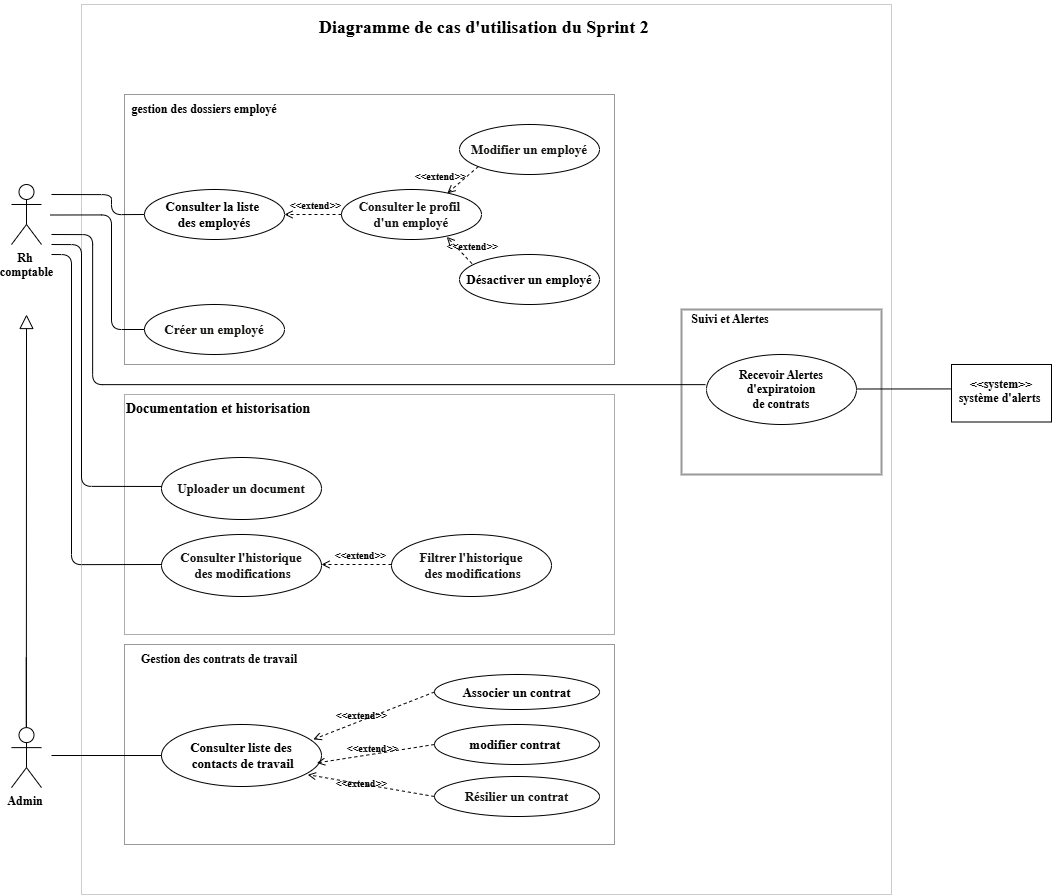
\includegraphics[width=0.95\textwidth]{use-case-sp2.png}
    \caption{Diagramme de cas d'utilisation du Sprint~2}
    \label{fig:use-case-sp2}
\end{figure}

Le diagramme de cas d'utilisation du Sprint~2 (Figure~\ref{fig:uc-sprint2})
  organise les fonctionnalités en trois packages fonctionnels distincts,
  reflétant les trois domaines couverts~: gestion du capital humain,
  gestion des contrats et gestion documentaire.

  \textbf{Relations UML~:} Le cas d'utilisation \og{}Consulter le profil
  employé\fg{} est en relation \texttt{<<include>>} avec
  \og{}Gérer les contrats\fg{} et \og{}Gérer les documents\fg{}, car le
  profil constitue le point d'entrée unique vers ces sous-modules. La
  relation de généralisation \textsc{Admin}~$\rightarrow$~\textsc{RH}
  héritée du Sprint~1 reste active~: l'Admin dispose de l'ensemble des
  droits du RH.

  \textbf{Responsabilités par acteur~:}

  \begin{itemize}
    \item \textbf{Admin Entreprise~:}
          Dispose de tous les droits du RH par héritage~; peut en sus
          superviser l'ensemble du personnel sans restriction de département.

    \item \textbf{RH Comptable~:}
          \begin{itemize}
            \item Gérer l'intégralité du dossier employé (créer, consulter,
                  modifier, désactiver).
            \item Associer, modifier et résilier les contrats de travail
                  (CDI, CDD, CIVP, KARAMA, Intérimaire, Stage).
            \item Déposer et consulter les documents administratifs
                  (\texttt{HrDocument}) dans le dossier employé.
            \item Consulter l'historique des modifications
                  (\texttt{EmployeeHistory}) pour tout dossier employé.
          \end{itemize}
  \end{itemize}

% -----------------------------------------------------------
\subsection{Description textuelle des cas d'utilisation}
% -----------------------------------------------------------

Les descriptions textuelles suivantes formalisent les préconditions,
scénarios nominaux et alternatifs des cas d'utilisation les plus
critiques du Sprint~2. Elles constituent la référence contractuelle de
validation avec le Product Owner.

% -----------------------------------------------------------
\subsubsection{Cas d'utilisation 1 : Créer un employé}
% -----------------------------------------------------------

Le tableau~\ref{tab:uc_creer_employe} présente la description textuelle
détaillée du cas d'utilisation «~Créer un employé~».
% ── CU 1 : Créer un employé ───────────────────────────────
\vspace{0.2cm}
\begin{xltabular}{\textwidth}{|l|X|}
    \hline
    \rowcolor[gray]{0.9} \textbf{Élément} & \textbf{Description} \\ \hline
    \endfirsthead
    \hline
    \rowcolor[gray]{0.9} \textbf{Élément} & \textbf{Description} \\ \hline
    \endhead
    \hline
    \endfoot
    \endlastfoot

    \textbf{Titre} & Créer un employé \\ \hline
    \textbf{Acteur principal} & Admin / RH Comptable \\ \hline
    \textbf{Préconditions} & L'utilisateur est authentifié (rôle Admin ou RH).
        Au moins un département et un poste actifs existent dans le système. \\ \hline
    \textbf{Postconditions} & Un nouveau profil employé est enregistré avec un
        matricule unique auto-généré. L'employé apparaît dans la liste du personnel
        de la société. L'action est tracée dans le journal d'audit. \\ \hline
    \textbf{Scénario principal} &
    \begin{enumerate}[nosep, leftmargin=*]
        \item L'acteur accède au formulaire de création d'un employé.
        \item Il renseigne les informations d'identité~: nom, prénom
              (en français et en arabe), date et lieu de naissance,
              genre, nationalité, numéro CIN, numéro CNSS.
        \item Il renseigne les informations fiscales et sociales~:
              situation familiale (\texttt{maritalStatus}), nombre
              d'enfants à charge (\texttt{numberOfChildren}), statut
              de chef de famille (\texttt{chefDeFamille}) ---
              ces données conditionnent le calcul de l'IRPP.
        \item Il renseigne les informations de contact~: adresse,
              ville, e-mail professionnel, téléphone, RIB bancaire.
        \item Il sélectionne le département, le poste et la catégorie
              de l'employé.
        \item Il renseigne la date d'embauche et la date de fin de
              période d'essai (optionnelle).
        \item Le système valide toutes les données saisies.
        \item Le système génère un matricule unique (format~: préfixe
              société + séquence auto-incrémentée).
        \item Le profil est enregistré en base et un message de
              confirmation est affiché.
    \end{enumerate} \\ \hline
    \textbf{Scénarios alternatifs}
    & \textbf{A1~: Données obligatoires manquantes} $\rightarrow$
      Erreurs de validation affichées sur les champs concernés~;
      la création est bloquée. \\ \cline{2-2}
    & \textbf{A2~: CIN déjà enregistré} $\rightarrow$
      Le système affiche un message d'unicité~; la création est bloquée. \\ \cline{2-2}
    & \textbf{A3~: Département ou poste inactif} $\rightarrow$
      Message d'erreur indiquant que la structure organisationnelle
      sélectionnée est inactive. \\ \hline
    \caption{Description textuelle du CU~: Créer un employé}
    \label{tab:uc_creer_employe}
\end{xltabular}
% -----------------------------------------------------------
\subsubsection{Cas d'utilisation 2 : Gérer les contrats de travail}
% -----------------------------------------------------------

Le tableau~\ref{tab:uc_gestion_contrats} présente la description
textuelle détaillée du cas d'utilisation «~Gérer les contrats de
travail~».
% ── CU 2 : Gérer les contrats de travail ─────────────────
\vspace{0.2cm}
\begin{xltabular}{\textwidth}{|l|X|}
    \hline
    \rowcolor[gray]{0.9} \textbf{Élément} & \textbf{Description} \\ \hline
    \endfirsthead
    \hline
    \rowcolor[gray]{0.9} \textbf{Élément} & \textbf{Description} \\ \hline
    \endhead
    \hline
    \endfoot
    \endlastfoot

    \textbf{Titre} & Gérer les contrats de travail
        (Associer / Modifier / Résilier) \\ \hline
    \textbf{Acteur principal} & RH Comptable \\ \hline
    \textbf{Préconditions} & L'utilisateur est authentifié (rôle RH).
        L'employé cible est actif dans le système et ne possède pas de
        contrat actif (pour une association). \\ \hline
    \textbf{Postconditions} & Le contrat est créé, modifié ou résilié.
        L'action est enregistrée dans le journal d'audit. \\ \hline
    \textbf{Scénario principal} &
    \begin{enumerate}[nosep, leftmargin=*]
        \item Le RH accède au profil de l'employé, onglet «~Contrats~».
        \item Il sélectionne l'action souhaitée~: association,
              modification ou résiliation.
        \item \textbf{Association~:} il sélectionne le type de contrat
              parmi les six types tunisiens supportés~:
              \textbf{CDI}, \textbf{CDD},
              \textbf{CIVP}, \textbf{KARAMA}, \textbf{Intérimaire} ou \textbf{Stage}~;
              il renseigne les conditions (date de début, salaire brut
              de base, heures hebdomadaires, convention collective)
              et confirme.
        \item \textbf{Modification~:} il met à jour les champs autorisés
              sur le contrat actif (hors type et date de début) et confirme.
        \item \textbf{Résiliation~:} il renseigne le motif de résiliation
              (champ obligatoire) et la date effective, puis confirme.
        \item Le système valide, applique les changements, met à jour
              le statut (ACTIF ~$\rightarrow$~ RÉSILIÉ)
              et enregistre l'action en base.
        \item Un message de confirmation est affiché.
    \end{enumerate} \\ \hline
    \textbf{Scénarios alternatifs}
    & \textbf{A1~: Contrat actif déjà existant} $\rightarrow$
      Le système bloque la création et affiche un message d'erreur. \\ \cline{2-2}
    & \textbf{A2~: Date de fin antérieure à la date de début (CDD)}
      $\rightarrow$ Erreur de validation bloquante. \\ \cline{2-2}
    & \textbf{A3~: Motif de résiliation absent} $\rightarrow$
      Erreur de validation~; le champ est obligatoire. \\ \cline{2-2}
    & \textbf{A4~: Durée CIVP dépassant 12~mois} $\rightarrow$
      Le système alerte que ce type de contrat est limité à un an. \\ \hline
    \caption{Description textuelle du CU~: Gérer les contrats de travail}
    \label{tab:uc_gestion_contrats}
\end{xltabular}
% -----------------------------------------------------------
\subsubsection{Cas d'utilisation 3 : Déposer un document administratif}
% -----------------------------------------------------------

Le tableau~\ref{tab:uc_deposer_document} présente la description
textuelle détaillée du cas d'utilisation «~Déposer un document
administratif~».
% ── CU 3 : Déposer un document administratif ─────────────
\vspace{0.2cm}
\begin{xltabular}{\textwidth}{|l|X|}
    \hline
    \rowcolor[gray]{0.9} \textbf{Élément} & \textbf{Description} \\ \hline
    \endfirsthead
    \hline
    \rowcolor[gray]{0.9} \textbf{Élément} & \textbf{Description} \\ \hline
    \endhead
    \hline
    \endfoot
    \endlastfoot

    \textbf{Titre} & Déposer un document administratif \\ \hline
    \textbf{Acteur principal} & RH \\ \hline
    \textbf{Préconditions} & L'utilisateur est authentifié avec le rôle RH.
        L'employé cible est enregistré dans le système. \\ \hline
    \textbf{Postconditions} & Le document est stocké et associé au dossier
        de l'employé. Le dépôt est tracé automatiquement dans le journal
        d'audit. \\ \hline
    \textbf{Scénario principal} &
    \begin{enumerate}[nosep, leftmargin=*]
        \item Le RH accède au profil de l'employé, section «~Documents~».
        \item Il clique sur «~Ajouter un document~».
        \item Il sélectionne le type de document (CONTRAT, ATTESTATION,
              DIPLOME, AUTRE).
        \item Il joint le fichier à déposer.
        \item Le système valide le format et la taille du fichier.
        \item Le document est enregistré avec ses métadonnées
              (type, auteur, horodatage).
        \item Un message de confirmation est affiché.
    \end{enumerate} \\ \hline
    \textbf{Scénarios alternatifs}
    & \textbf{A1~: Format de fichier non supporté} $\rightarrow$
      Un message d'erreur liste les formats acceptés~;
      le dépôt est bloqué. \\ \cline{2-2}
    & \textbf{A2~: Taille du fichier dépassant la limite autorisée}
      $\rightarrow$ Un message d'erreur indique la taille maximale
      autorisée~; le dépôt est bloqué. \\ \hline
    \caption{Description textuelle du CU~: Déposer un document administratif}
    \label{tab:uc_deposer_document}
\end{xltabular}

% ============================================================
\section{Conception du deuxième Sprint}
\label{sec:s2-conception}
% ============================================================

La conception technique du Sprint~2 traduit les besoins métiers en
modèles structurants guidant le développement. Cette section s'articule
autour de deux axes complémentaires~: le diagramme de classes, qui
modélise l'architecture statique des nouvelles entités, et les
diagrammes de séquence, qui illustrent les interactions dynamiques entre
les composants du système.

% -----------------------------------------------------------
\subsection{Diagramme de classes}
% -----------------------------------------------------------

Le diagramme de classes du Sprint~2 étend le modèle établi lors du
Sprint~1 en introduisant les nouvelles entités du domaine RH. Il définit
la structure des données --- employés, contrats et documents
--- ainsi que les relations de dépendance qui les unissent avec les
entités existantes (UserProfile, Company, Department,JobPosition).

La figure~\ref{fig:classes-sprint2} présente le diagramme de classes du
Sprint~2, illustrant l'extension du modèle de données.

\begin{figure}[H]
    \centering
    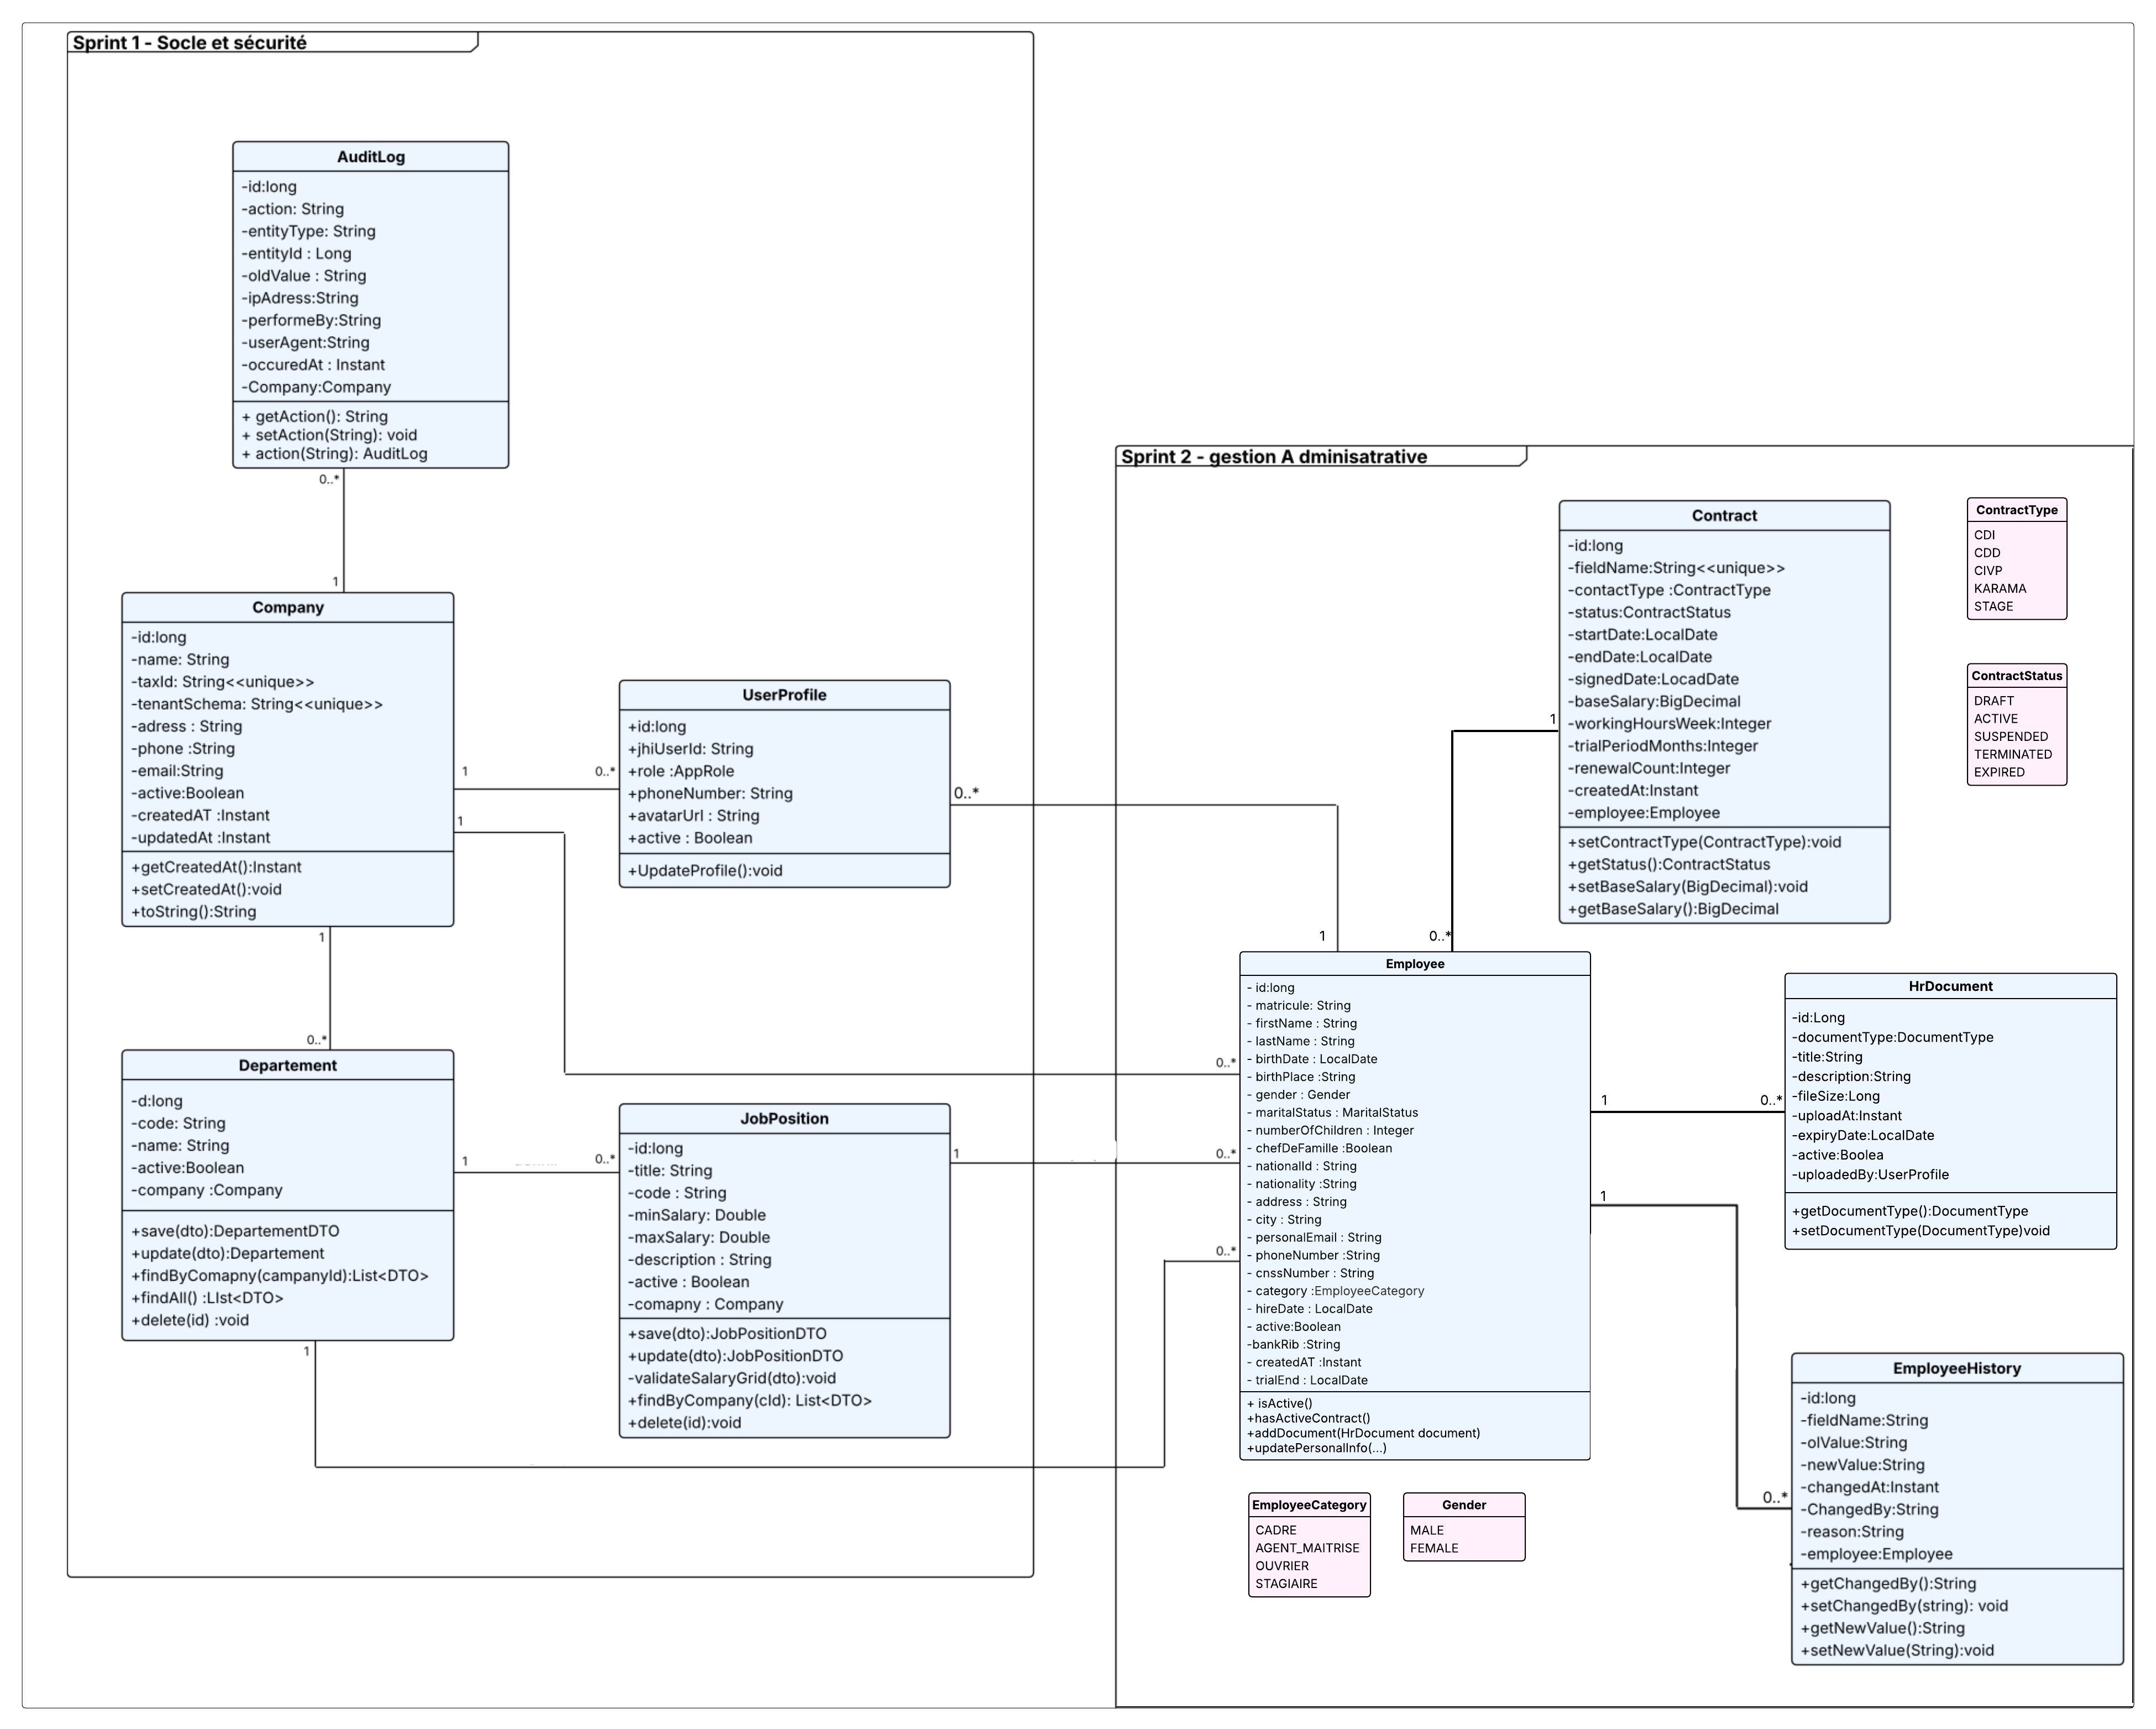
\includegraphics[width=1\textwidth]{classes-sprint2}
    \caption{Diagramme de classes du Sprint~2}
    \label{fig:classes-sprint2}
\end{figure}

Les entités principales introduites dans ce sprint sont les suivantes~:

\begin{itemize}
    \item \textbf{Employee}~: entité centrale du sprint.
          Outre les informations d'identité (matricule, nom, prénom, CIN,
          date de naissance, genre, nationalité, numéro CNSS), elle stocke
          les données fiscales et sociales indispensables au moteur de paie
          du Sprint~3~: la situation familiale, le nombre d'enfants à charge,
          le statut de chef de famille (déductible IRPP), le RIB bancaire
          pour virement et le solde de congés. Elle est associée à la société,
          au département et au poste, et peut être liée au compte
          d'authentification de l'utilisateur. Une auto-association
          optionnelle modélise la relation hiérarchique entre un employé
          et son responsable.

    \item \textbf{Contract}~: représente le contrat de travail d'un employé.
          Elle porte une référence unique, le type de contrat (CDI, CDD,
          CIVP, KARAMA, Intérimaire, Stage), le statut (actif, résilié
          ou suspendu), les dates clés (début et fin), le salaire brut
          de base, la durée hebdomadaire de travail, la convention
          collective applicable et la durée de la période d'essai.

    \item \textbf{HrDocument}~: modélise les pièces administratives attachées
          au dossier d'un employé (CV, diplômes, scans de contrats,
          attestations manuelles). Elle est identifiée par son type
          (contrat, attestation, diplôme ou autre), son titre et les
          métadonnées de dépôt (auteur, horodatage, taille).
\end{itemize}
% -----------------------------------------------------------
\subsection{Diagrammes de séquences}
% -----------------------------------------------------------

Les diagrammes de séquences illustrent la dynamique du système en
détaillant les interactions chronologiques entre les composants pour
les cas d'utilisation les plus critiques.

\subsubsection{Diagramme de séquence : Création d'un employé}

La figure~\ref{fig:seq-create-employe} illustre le flux de création
d'un employé dans PaieZone, incluant la génération du matricule et le
déclenchement automatique de l'enregistrement dans l'historique.

\begin{figure}[H]
    \centering
    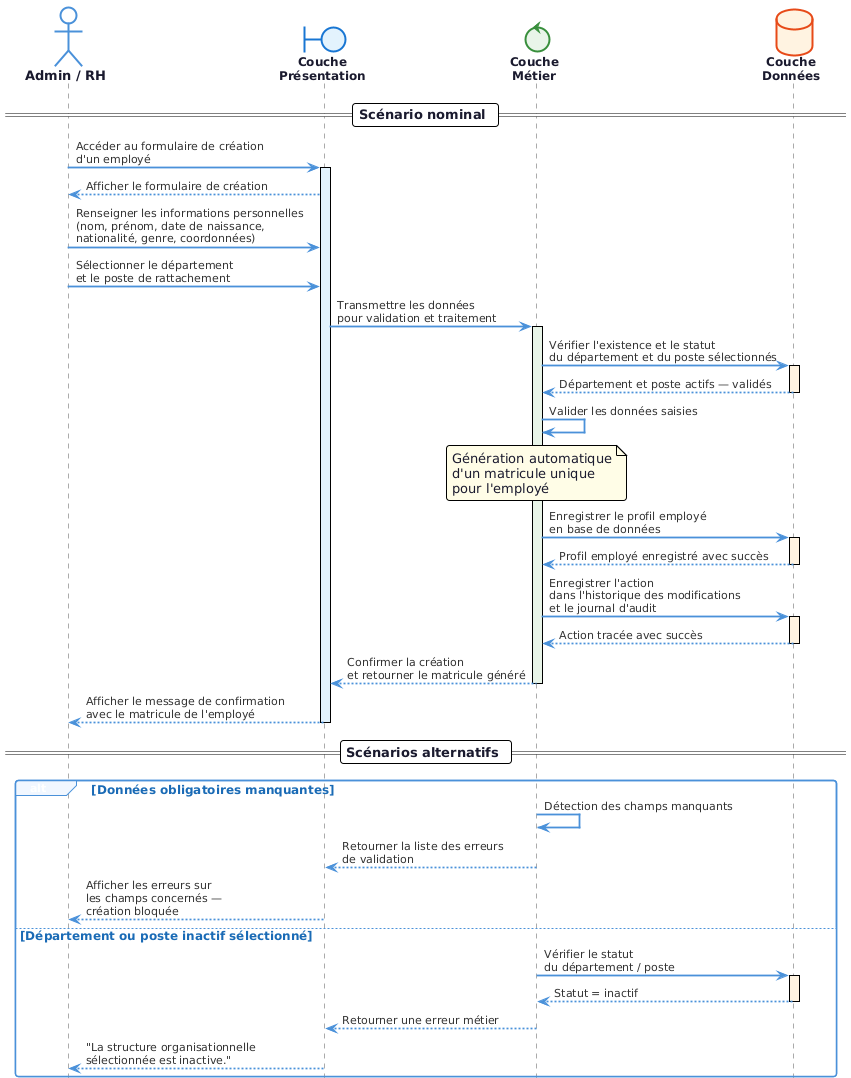
\includegraphics[width=0.91\textwidth]{seq-sp2-uc1.png}
    \caption{Diagramme de séquence --- Création d'un employé}
    \label{fig:seq-create-employe}
\end{figure}
\subsubsection{Diagramme de séquence : Association d'un contrat}

La figure~\ref{fig:seq-create-contrat} illustre le flux d'association
d'un contrat de travail à un employé dans PaieZone, incluant les
validations métier et la mise à jour du statut.

\begin{figure}[H]
    \centering
    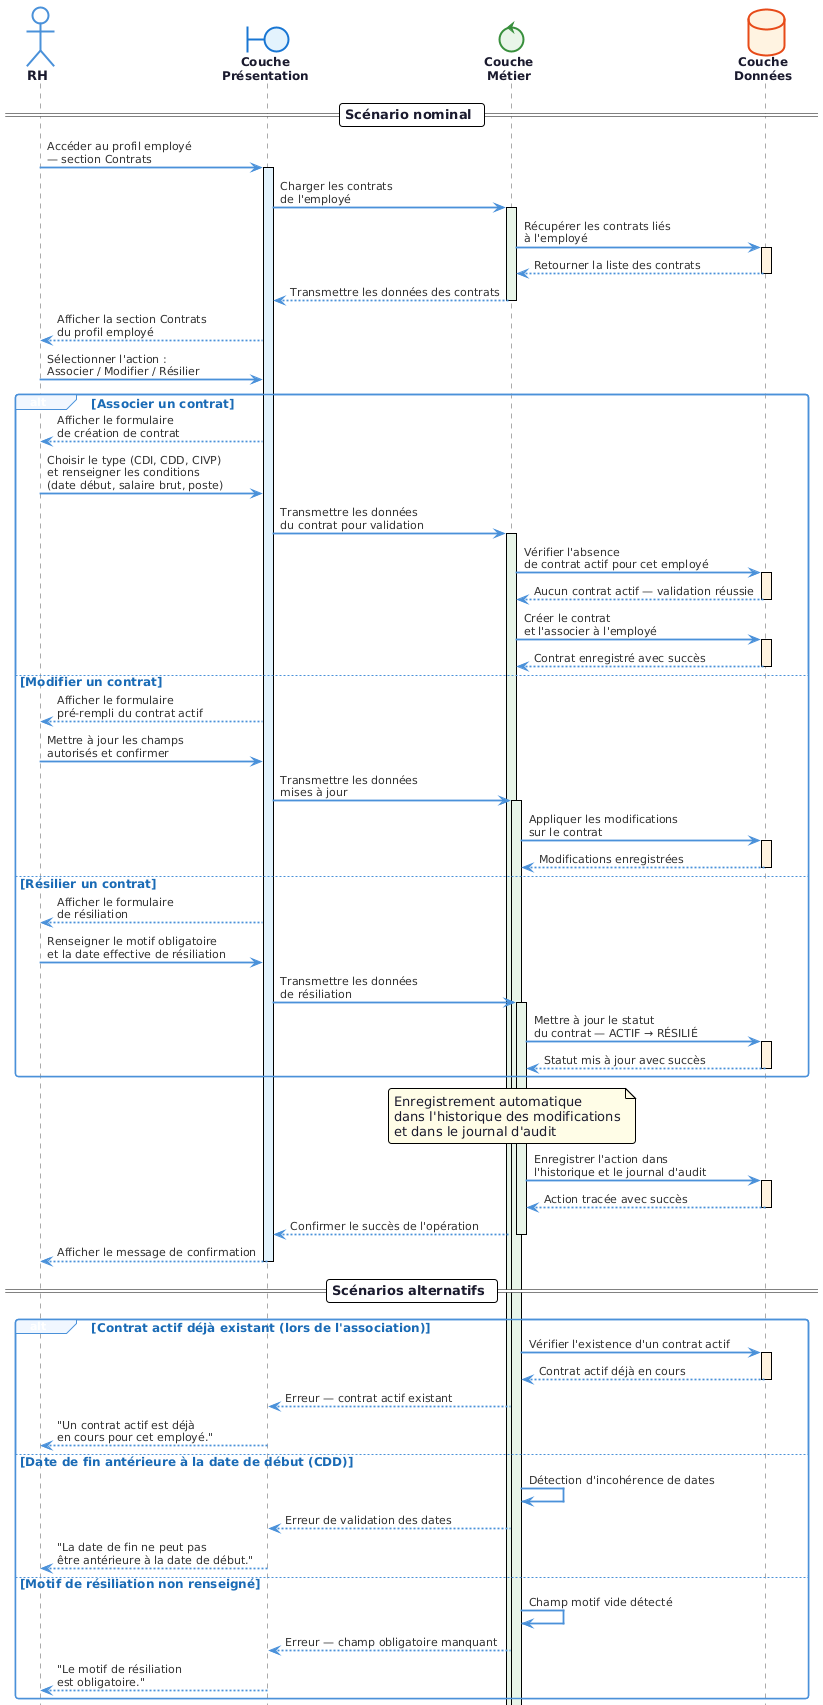
\includegraphics[width=0.69\textwidth]{seq-sp2-uc2.png}
    \caption{Diagramme de séquence --- Association d'un contrat à un
             employé}
    \label{fig:seq-create-contrat}
\end{figure}



% ============================================================
\section{Étude et réalisation du deuxième sprint}
\label{sec:s2-realisation}
% ============================================================

Cette section présente les réalisations concrètes du Sprint~2, marquant
le passage des spécifications à des fonctionnalités opérationnelles
livrées. Les travaux ont porté sur l'implémentation du module de gestion
des employés, le cycle de vie des contrats de travail, la gestion
documentaire et le système d'historisation. Ces développements
matérialisent la validation des 10 User Stories planifiées et
constituent le c\oe{}ur métier RH de la plateforme PaieZone.

% -----------------------------------------------------------
\subsection{Gestion des employés}
% -----------------------------------------------------------

Le module de gestion des employés constitue l'épine dorsale du
Sprint~2. Il offre à l'équipe RH et aux Administrateurs un contrôle
complet sur les dossiers du personnel de la société.

\begin{figure}[H]
    \centering
    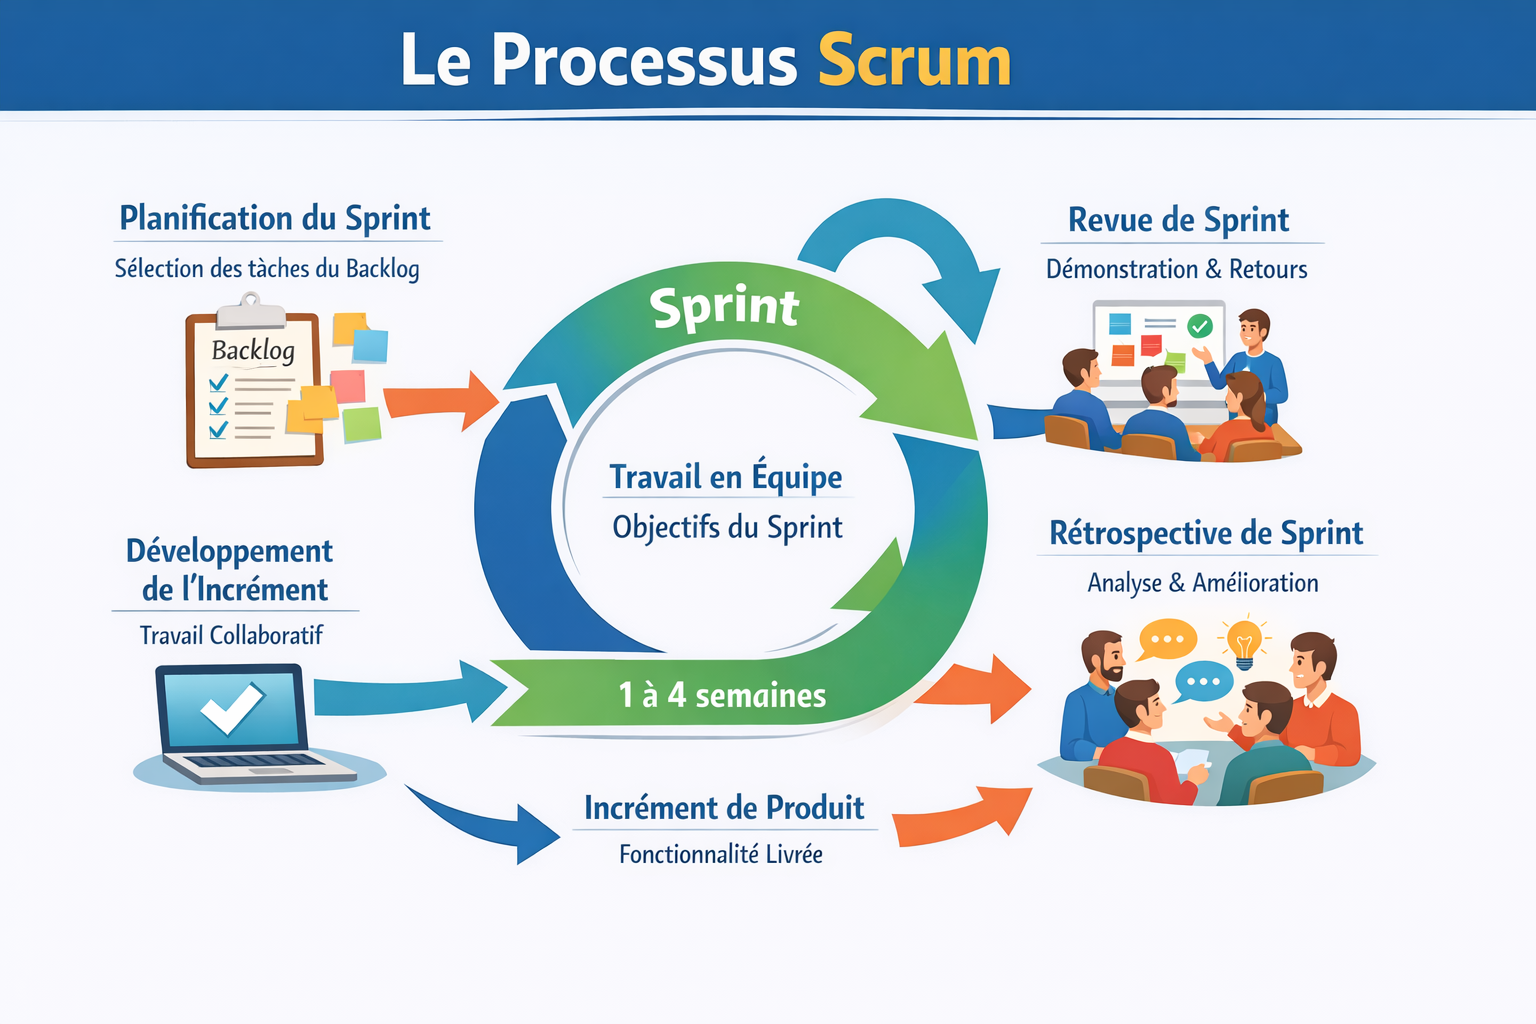
\includegraphics[width=0.70\textwidth]{scrum.png}
    \caption{Liste des employés --- Vue d'ensemble du personnel}
    \label{fig:ui-employees-list}
\end{figure}

La figure~\ref{fig:ui-employees-list} illustre l'interface de
consultation de la liste des employés. Les collaborateurs sont présentés
avec leurs informations clés~: matricule, identité, département, poste
et statut. La table intègre des fonctions de recherche multicritère et
de pagination pour faciliter la navigation au sein des effectifs.

\newpage

\begin{figure}[H]
    \centering
    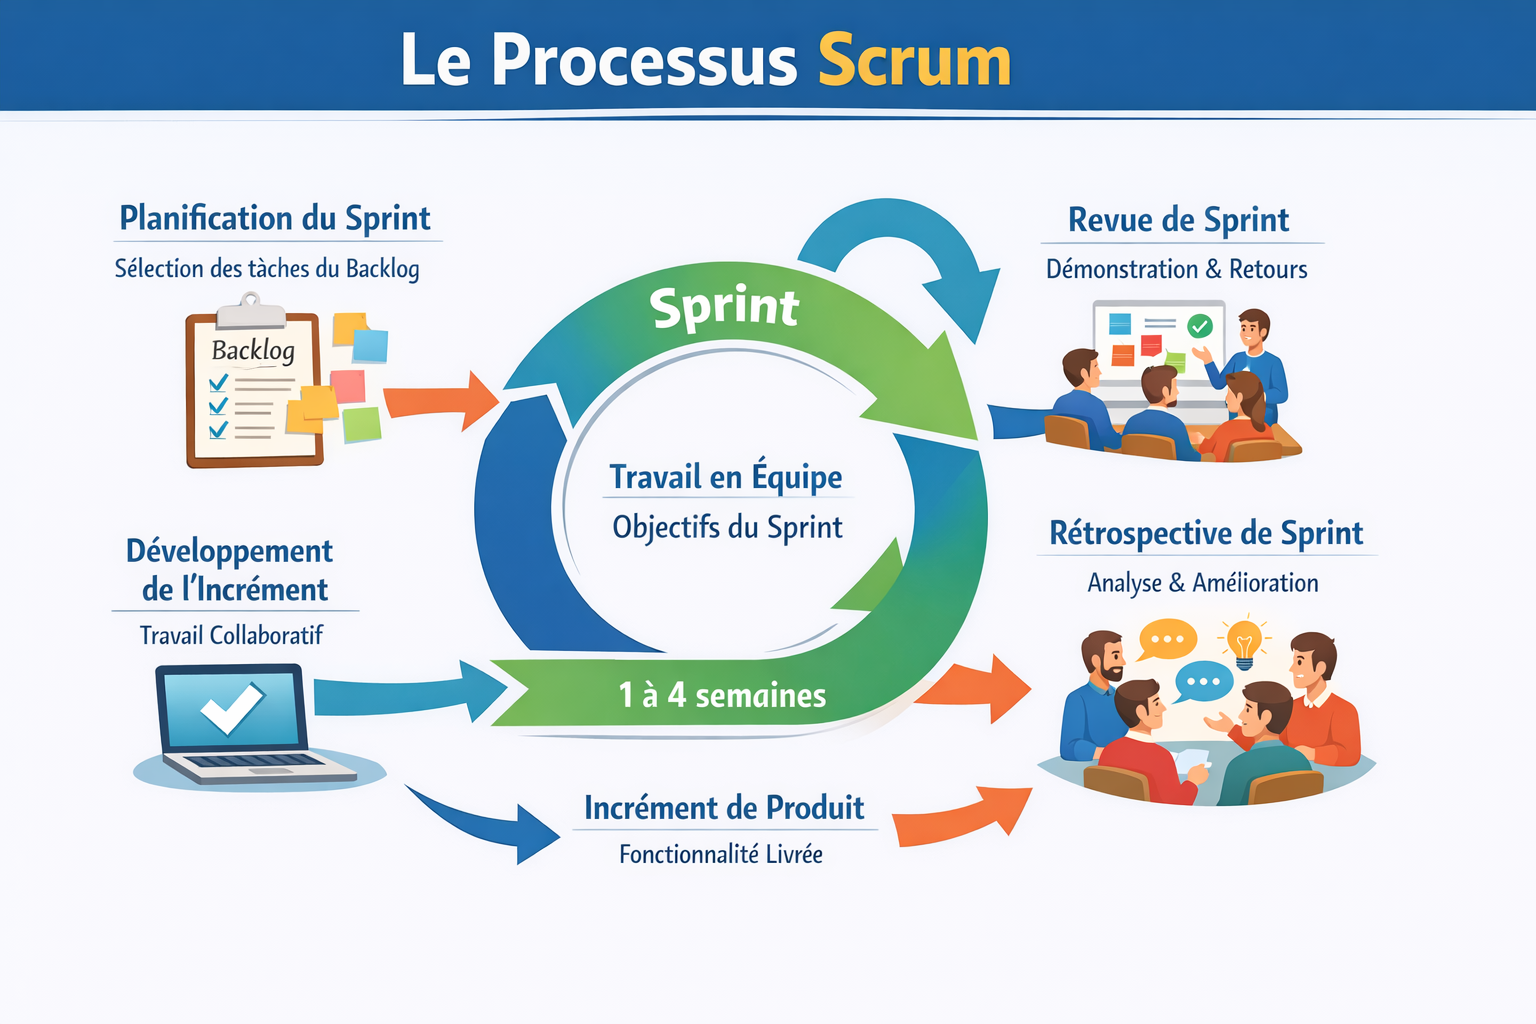
\includegraphics[width=0.70\textwidth]{scrum.png}
    \caption{Formulaire de création et de modification d'un employé}
    \label{fig:ui-employee-form}
\end{figure}

La Figure~\ref{fig:ui-employee-form} présente l'interface dédiée à la gestion 
des dossiers employés. Ce formulaire permet de renseigner l'ensemble des informations personnelles, fiscales et administratives nécessaires au suivi du collaborateur. Pour garantir la fiabilité du système, chaque saisie fait l'objet d'un contrôle automatique rigoureux, empêchant ainsi les erreurs de format ou la création de profils en double.

\begin{figure}[H]
    \centering
    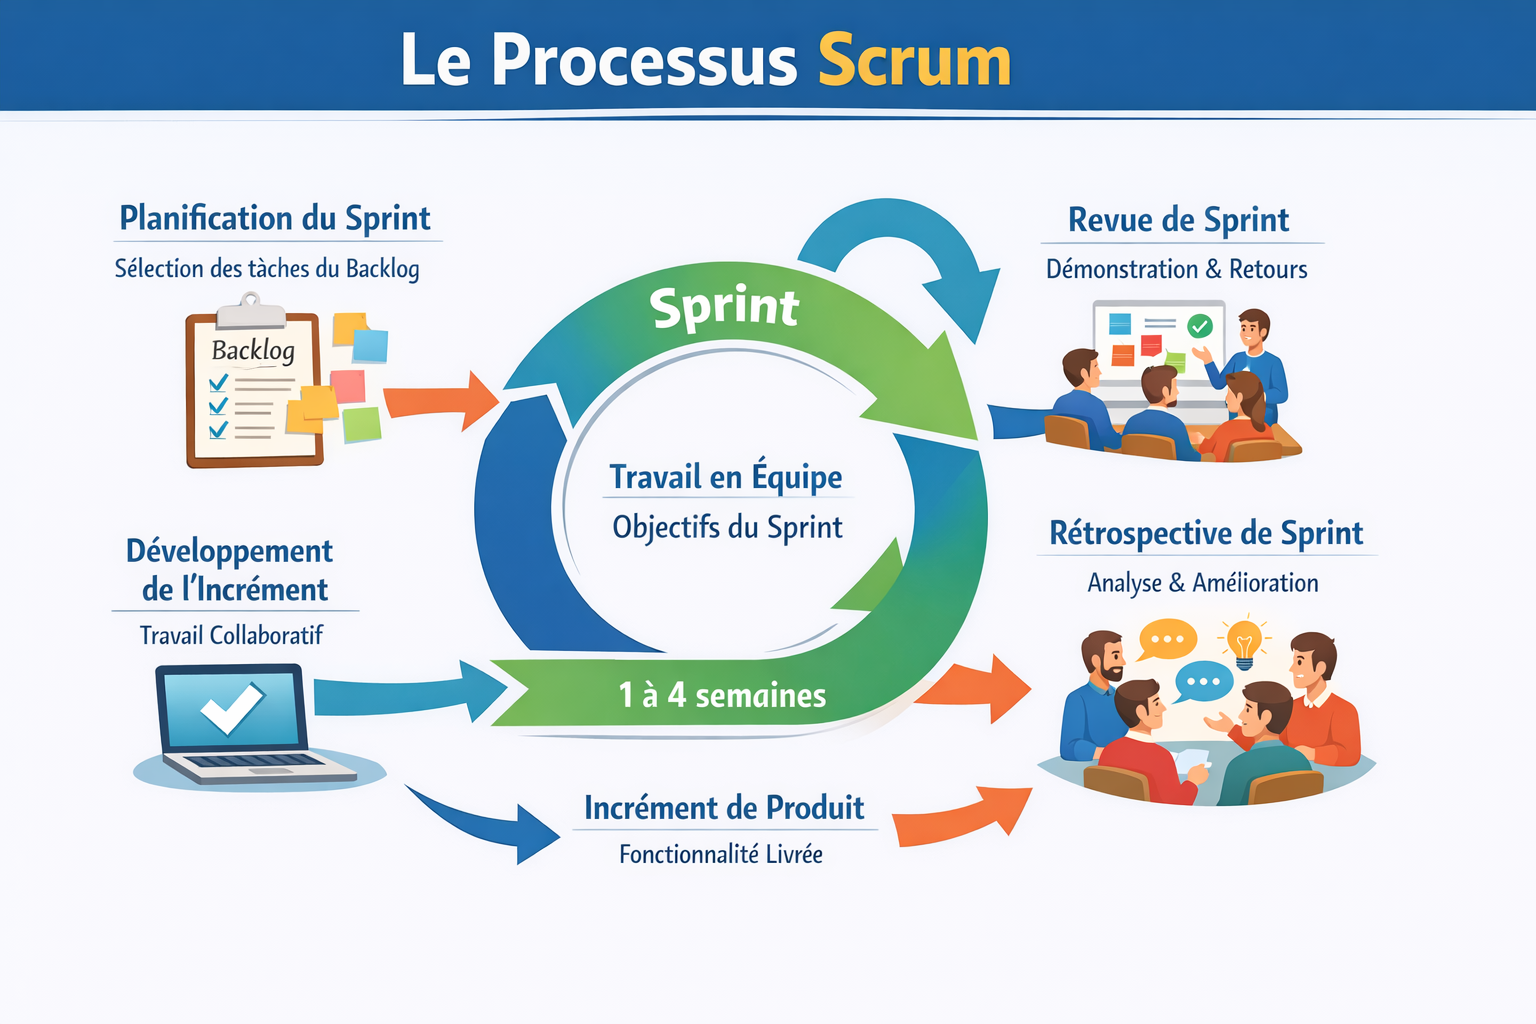
\includegraphics[width=0.70\textwidth]{scrum.png}
    \caption{Vue détaillée du profil employé}
    \label{fig:ui-employee-profile}
\end{figure}

La figure~\ref{fig:ui-employee-profile} illustre la vue détaillée du
profil d'un employé, centralisant l'ensemble de son dossier
administratif~: informations personnelles, contrats associés, documents
stockés et historique des modifications. Cette vue constitue le point
d'entrée unique pour toutes les opérations liées au dossier d'un
collaborateur.

% -----------------------------------------------------------
\subsection{Gestion des contrats de travail}
% -----------------------------------------------------------

Le module de gestion des contrats formalise la relation de travail entre
l'employé et la société. Il couvre l'intégralité du cycle de vie
contractuel~: association, modification et résiliation.

\begin{figure}[H]
    \centering
    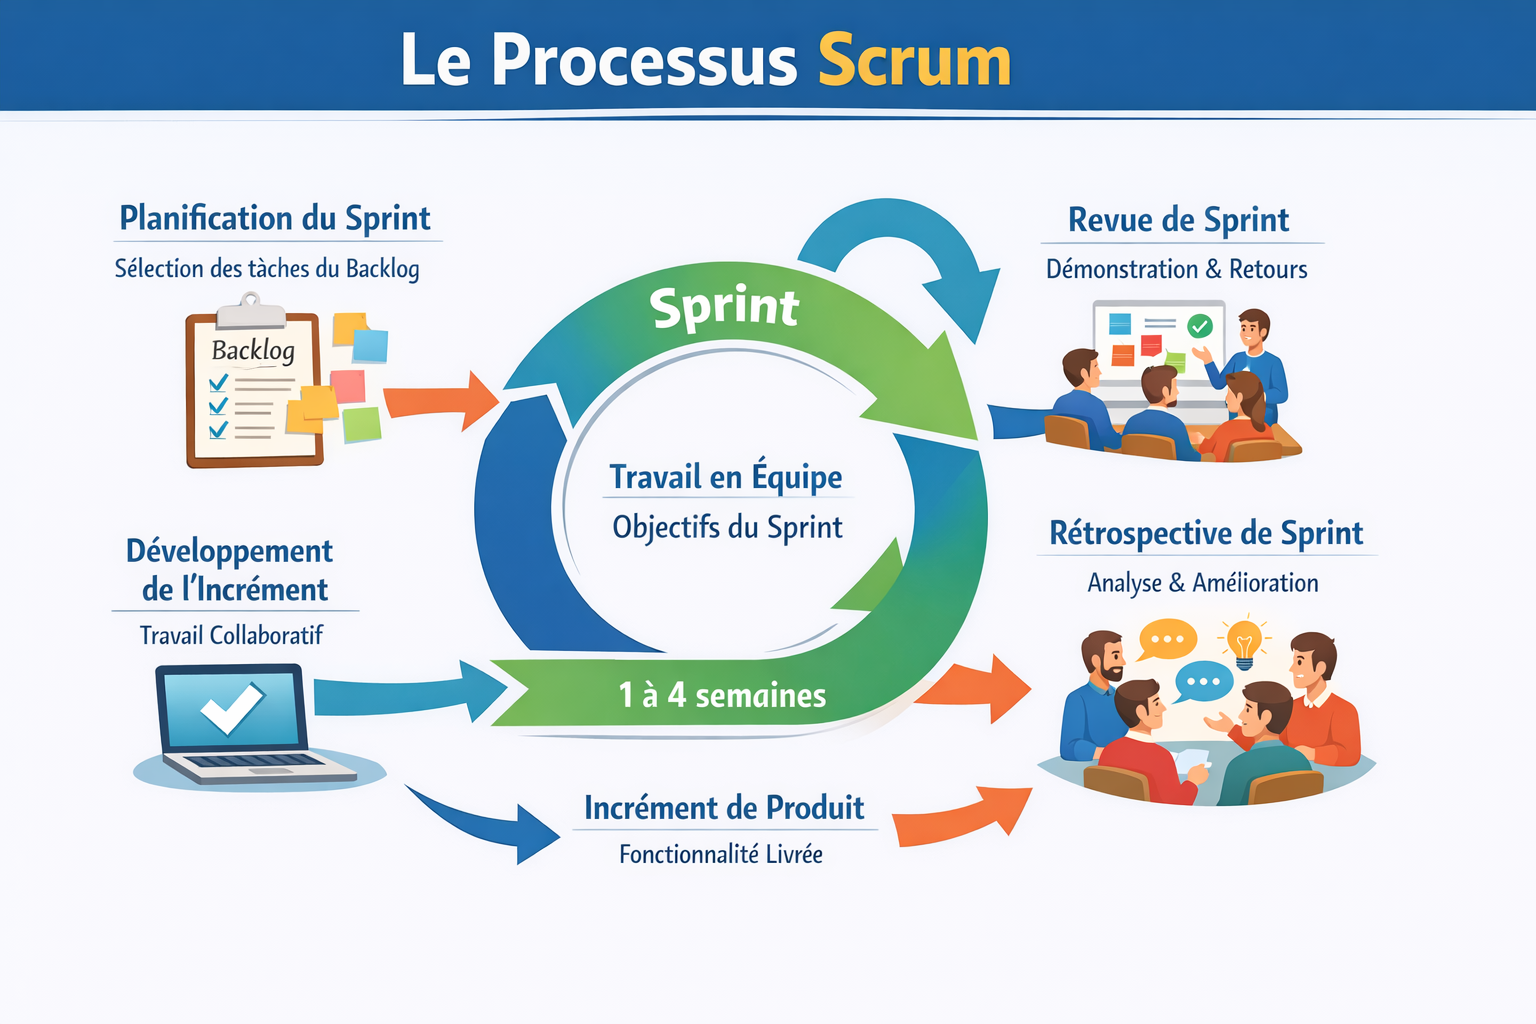
\includegraphics[width=0.70\textwidth]{scrum.png}
    \caption{Section Contrats du dossier employé}
    \label{fig:ui-contracts-list}
\end{figure}

La figure~\ref{fig:ui-contracts-list} présente la section «~Contrats~»
du dossier employé, affichant l'historique contractuel avec le type, le
statut, les dates clés et le salaire brut. Les actions disponibles
(modifier, résilier) sont conditionnées au statut courant du contrat,
empêchant toute opération incohérente.

% -----------------------------------------------------------
\subsection{Gestion des documents administratifs}
% -----------------------------------------------------------

Le module de gestion documentaire permet à l'équipe RH de constituer un
dossier numérique complet pour chaque employé, en stockant de manière
sécurisée l'ensemble des pièces administratives.
\newpage

\begin{figure}[H]
    \centering
    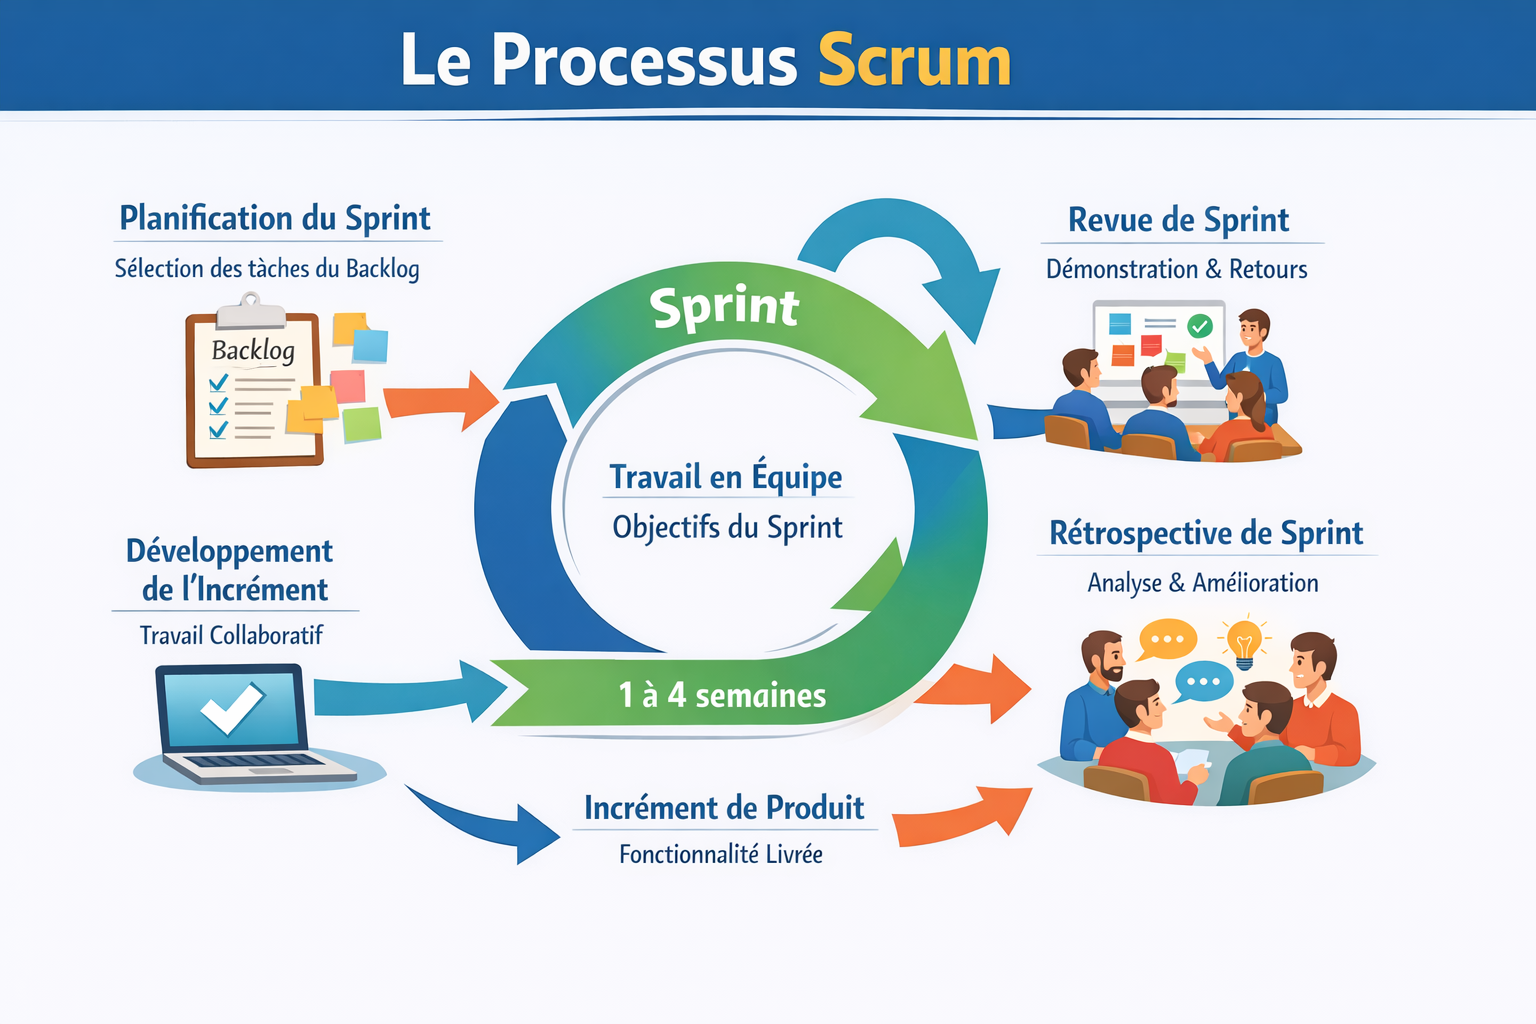
\includegraphics[width=0.70\textwidth]{scrum.png}
    \caption{Section Documents du dossier employé --- Dépôt et
             consultation}
    \label{fig:ui-documents}
\end{figure}

La figure~\ref{fig:ui-documents} présente la section «~Documents~» du
dossier employé. Le RH peut déposer des fichiers en sélectionnant leur
type parmi une liste prédéfinie (CONTRAT, ATTESTATION, DIPLOME, AUTRE).
Chaque document est référencé avec son nom, son type et la date de dépôt.


% ============================================================
\section{Tests et Validation}
\label{sec:s2-tests}
% ============================================================

La phase de tests et de validation du Sprint~2 vise à garantir la
conformité des fonctionnalités implémentées aux exigences des User
Stories et à assurer la robustesse des modules métier livrés. Trois
niveaux de tests ont été mis en œuvre de manière complémentaire.

% -----------------------------------------------------------
\subsection{Plan de tests}
% -----------------------------------------------------------

\begin{itemize}[label=\textbullet, leftmargin=0.6cm]
    \item \textbf{Tests unitaires :} Sécurisent les règles de gestion internes (statuts des contrats, formats documentaires).
    \item \textbf{Tests d'intégration:} Confirment l'interopérabilité entre les différents modules (employés, postes, contrats).
    \item \textbf{Tests fonctionnels:} Valident l'ergonomie des formulaires et la fiabilité des affichages dynamiques sous Angular.
\end{itemize}
Cette démarche rigoureuse assure que chaque fonctionnalité développée est strictement conforme aux critères d'acceptation des User Stories. Le Tableau~\ref{tab:tests-sprint2} récapitule les principaux scénarios de test exécutés, confirmant ainsi la stabilité et la validité du système pour ce sprint.
principaux réalisés pour ce sprint.
\renewcommand{\arraystretch}{1.3}
\begin{xltabular}{\textwidth}{|p{1.5cm}|X|p{4cm}|p{1.5cm}|}
\hline
\rowcolor[gray]{0.9}
\textbf{ID} & \textbf{Description} & \textbf{Résultat attendu} & \textbf{Statut} \\ \hline
\endfirsthead
\hline
\rowcolor[gray]{0.9}
\textbf{ID} & \textbf{Description} & \textbf{Résultat attendu} & \textbf{Statut} \\ \hline
\endhead
\hline
\endfoot
\hline
\caption{Récapitulatif des cas de test du Sprint~2}
\label{tab:tests-sprint2}
\endlastfoot

T-6.1 & Création d'un employé avec tous les champs valides
       & Employé créé avec matricule auto-généré, persisté en base
       & \textcolor{green!60!black}{\textbf{OK}} \\ \hline

T-6.2 & Création d'un employé avec CIN déjà existant
       & Erreur d'unicité, création bloquée
       & \textcolor{green!60!black}{\textbf{OK}} \\ \hline

T-6.3 & Désactivation d'un employé possédant un contrat actif
       & Avertissement affiché, désactivation conditionnelle
       & \textcolor{green!60!black}{\textbf{OK}} \\ \hline

T-7.1 & Association d'un contrat CDI à un employé sans contrat actif
       & Contrat créé avec statut ACTIF
       & \textcolor{green!60!black}{\textbf{OK}} \\ \hline

T-7.2 & Association d'un contrat CIVP avec une durée supérieure à 12~mois
       & Alerte de durée maximale affichée
       & \textcolor{green!60!black}{\textbf{OK}} \\ \hline

T-7.3 & Tentative d'association d'un second contrat actif sur un employé
        déjà sous contrat
       & Blocage avec message d'erreur explicite
       & \textcolor{green!60!black}{\textbf{OK}} \\ \hline

T-7.4 & Résiliation d'un contrat sans motif renseigné
       & Erreur de validation, résiliation bloquée
       & \textcolor{green!60!black}{\textbf{OK}} \\ \hline

T-8.1 & Dépôt d'un fichier PDF valide dans le dossier employé
       & Document enregistré et visible dans la liste des documents
       & \textcolor{green!60!black}{\textbf{OK}} \\ \hline

T-8.2 & Dépôt d'un fichier de format non supporté (ex.~: .exe)
       & Rejet avec message listant les formats acceptés
       & \textcolor{green!60!black}{\textbf{OK}} \\ \hline

\end{xltabular}
\renewcommand{\arraystretch}{1.0}

% -----------------------------------------------------------
\subsection{Tests automatisés}
% -----------------------------------------------------------

Pour le Sprint~2, les tests automatisés ont ciblé le flux d'approbation
des avances sur salaire --- l'un des processus métier à changements d'état
les plus sensibles de la plateforme.

\paragraph{Tests unitaires --- AdvanceWorkflowTest (JUnit~5 + Mockito)}
Quatre cas de test valident les transitions d'état du service \texttt{AdvanceServiceImpl}~:

\renewcommand{\arraystretch}{1.2}
\begin{small}
\begin{xltabular}{\textwidth}{|c|X|p{4cm}|c|}
\hline
\rowcolor[gray]{0.9}
\textbf{ID} & \textbf{Scénario} & \textbf{Résultat attendu} & \textbf{Statut} \\ \hline
\endfirsthead \hline
\rowcolor[gray]{0.9}
\textbf{ID} & \textbf{Scénario} & \textbf{Résultat attendu} & \textbf{Statut} \\ \hline
\endhead \hline \endfoot \hline
\caption{Tests automatisés --- AdvanceWorkflowTest}\label{tab:auto-s2}\endlastfoot
TA-S2-01 & Approbation d'une avance au statut \texttt{REQUESTED}
    & Statut passe à \texttt{APPROVED} & \textcolor{green!60!black}{\textbf{OK}} \\ \hline
TA-S2-02 & Refus d'une avance au statut \texttt{REQUESTED}
    & Statut passe à \texttt{REJECTED} & \textcolor{green!60!black}{\textbf{OK}} \\ \hline
TA-S2-03 & Approbation d'une avance déjà \texttt{APPROVED}
    & Exception levée (\textit{transition interdite}) & \textcolor{green!60!black}{\textbf{OK}} \\ \hline
TA-S2-04 & Avance introuvable en base
    & Exception \texttt{404 Not Found} & \textcolor{green!60!black}{\textbf{OK}} \\ \hline
\end{xltabular}
\end{small}
\renewcommand{\arraystretch}{1.0}

\textbf{Résultat~:} 4/4 tests passés (\textcolor{green!60!black}{\textbf{OK}}).

% ============================================================
\section{Rituels Agiles et Clôture du Sprint}
\label{sec:s2-rituels}
% ============================================================

Conformément à la méthodologie Scrum adoptée par l'équipe PaieZone,
le Sprint~2 s'est clôturé par la tenue des deux rituels essentiels~:
la Sprint Review et la Sprint Retrospective. Ces cérémonies assurent
la transparence du travail accompli et l'amélioration continue des
pratiques d'équipe.
% -----------------------------------------------------------
\subsection{Revue du Sprint (Sprint Review)}
% -----------------------------------------------------------

La Sprint Review a réuni l'équipe de développement, le Product Owner
et les parties prenantes. Les démonstrations ont couvert la gestion
du capital humain (création, modification et désactivation des profils
employés), l'association des six types de contrats tunisiens (CDI, CDD,
CIVP, KARAMA, Intérimaire et Stage), ainsi que le dépôt et la
consultation des documents administratifs. L'ensemble des 9 User
Stories planifiées a été validé par le Product Owner, confirmant la
conformité des livrables aux critères d'acceptation.
% -----------------------------------------------------------
\subsection{Rétrospective du Sprint (Sprint Retrospective)}
% -----------------------------------------------------------

La rétrospective a permis à l'équipe de réfléchir sur trois axes~:

\begin{itemize}[label=\textbullet, leftmargin=0.6cm]
    \item \textbf{Ce qui a bien fonctionné~:} La synergie entre les
          équipes front-end et back-end a garanti une livraison fluide
          des fonctionnalités. La réutilisation des composants Angular
          existants a accéléré le développement des interfaces de
          gestion des employés et des contrats.

    \item \textbf{Problèmes rencontrés~:} La gestion du stockage des
          fichiers (formats, tailles, types) a engendré des contraintes
          techniques imprévues, nécessitant des ajustements de la
          configuration du service de stockage en cours de sprint.

    \item \textbf{Actions d'amélioration pour le Sprint~3~:} Anticiper
          l'analyse des dépendances techniques entre les modules dès
          le début du sprint afin de réduire les blocages en cours de
          développement et de garantir une livraison dans les délais
          prévus.
\end{itemize}
\section*{Conclusion}
\label{sec:s2-conclusion}
\addcontentsline{toc}{section}{Conclusion}

Ce chapitre a détaillé la mise en œuvre du cœur métier RH de PaieZone RH. La validation des User Stories liées à la gestion des employés, des contrats tunisiens et de la GED (Gestion Électronique des Documents) a permis de consolider le référentiel de données avec les entités clés.

Ces acquis constituent le socle indispensable pour le Sprint 3 : les paramètres fiscaux et sociaux ainsi que les conditions contractuelles seront directement exploités par le moteur de calcul.

Le chapitre suivant sera consacré au Sprint 3, portant sur l'automatisation de la paie, les déclarations sociales et la gestion des absences.


